\section{Competitive Battling Track}

\subsection{Battling Environment Design}
\href{https://play.pokemonshowdown.com}{Pokémon Showdown} is an open-source simulator that transforms Pokémon's turn-based battle mechanics into a standalone competitive game with thousands of daily players. Formally, battles are two-player, zero-sum, stochastic games with imperfect information and simultaneous action selection. Their imperfect information primarily stems from team construction: each player drafts a team from a vast design space, and key aspects of the opponent’s team remain hidden until revealed through play. On each turn, players select from \textasciitilde9 actions (Figure \ref{fig:battle}), with battles lasting \textasciitilde20--100 turns. Action outcomes are stochastic and can lead to a long tail of rare events that abruptly swing state values. The combination of randomness, hidden information, team diversity, long-horizon planning, and evolving rules presents a significant challenge, and evaluating progress is difficult: existing work typically relies on disjoint baselines or anonymous competition on the Pokémon Showdown ranked ladder, where performance metrics are noisy and non-stationary. We address these challenges by releasing standardized baselines and datasets alongside a dedicated leaderboard for AI agents.


\subsection{Battling Evaluation Criteria}
\label{sec:track1:evaluation}

Battling Track agents are evaluated through direct competition against both community submissions and a diverse suite of state-of-the-art baselines maintained by our team. To avoid interfering with human players, all matches are conducted on a separate, modified Showdown server operated by the PokéAgent Challenge and configured specifically for AI benchmarking.


\vspace{-2mm}

\paragraph{Skill Rating Metrics.} Agents are ranked on a public leaderboard according to several metrics. We report the standard Showdown implementations of \textbf{Glicko-1}~\citep{glickman1999parameter} (an Elo variant incorporating uncertainty) and \textbf{GXE} (expected win probability against a randomly sampled opponent). However, these online metrics are designed for a large human player base with evolving skills and sparse matchups. In contrast, our agent pool is comparatively small, matchups are dense, and policies are fixed during evaluation. Our primary metric is based on a Bradley--Terry model~\citep{bradley1952rank} with bootstrapped uncertainty, fit over the full history of an agent’s battle results subject to a minimum sample size. We refer to this metric as the \textbf{Full-History Bradley--Terry} (\textbf{FH-BT}) rating to distinguish it from Showdown’s version of Elo, which is too noisy for our purposes. Appendix \ref{sec:track1-full-results} provides a comparison of alternative skill metrics.

\begin{wrapfigure}{r}{0.30\linewidth}
    \centering
    \vspace{-10mm}
    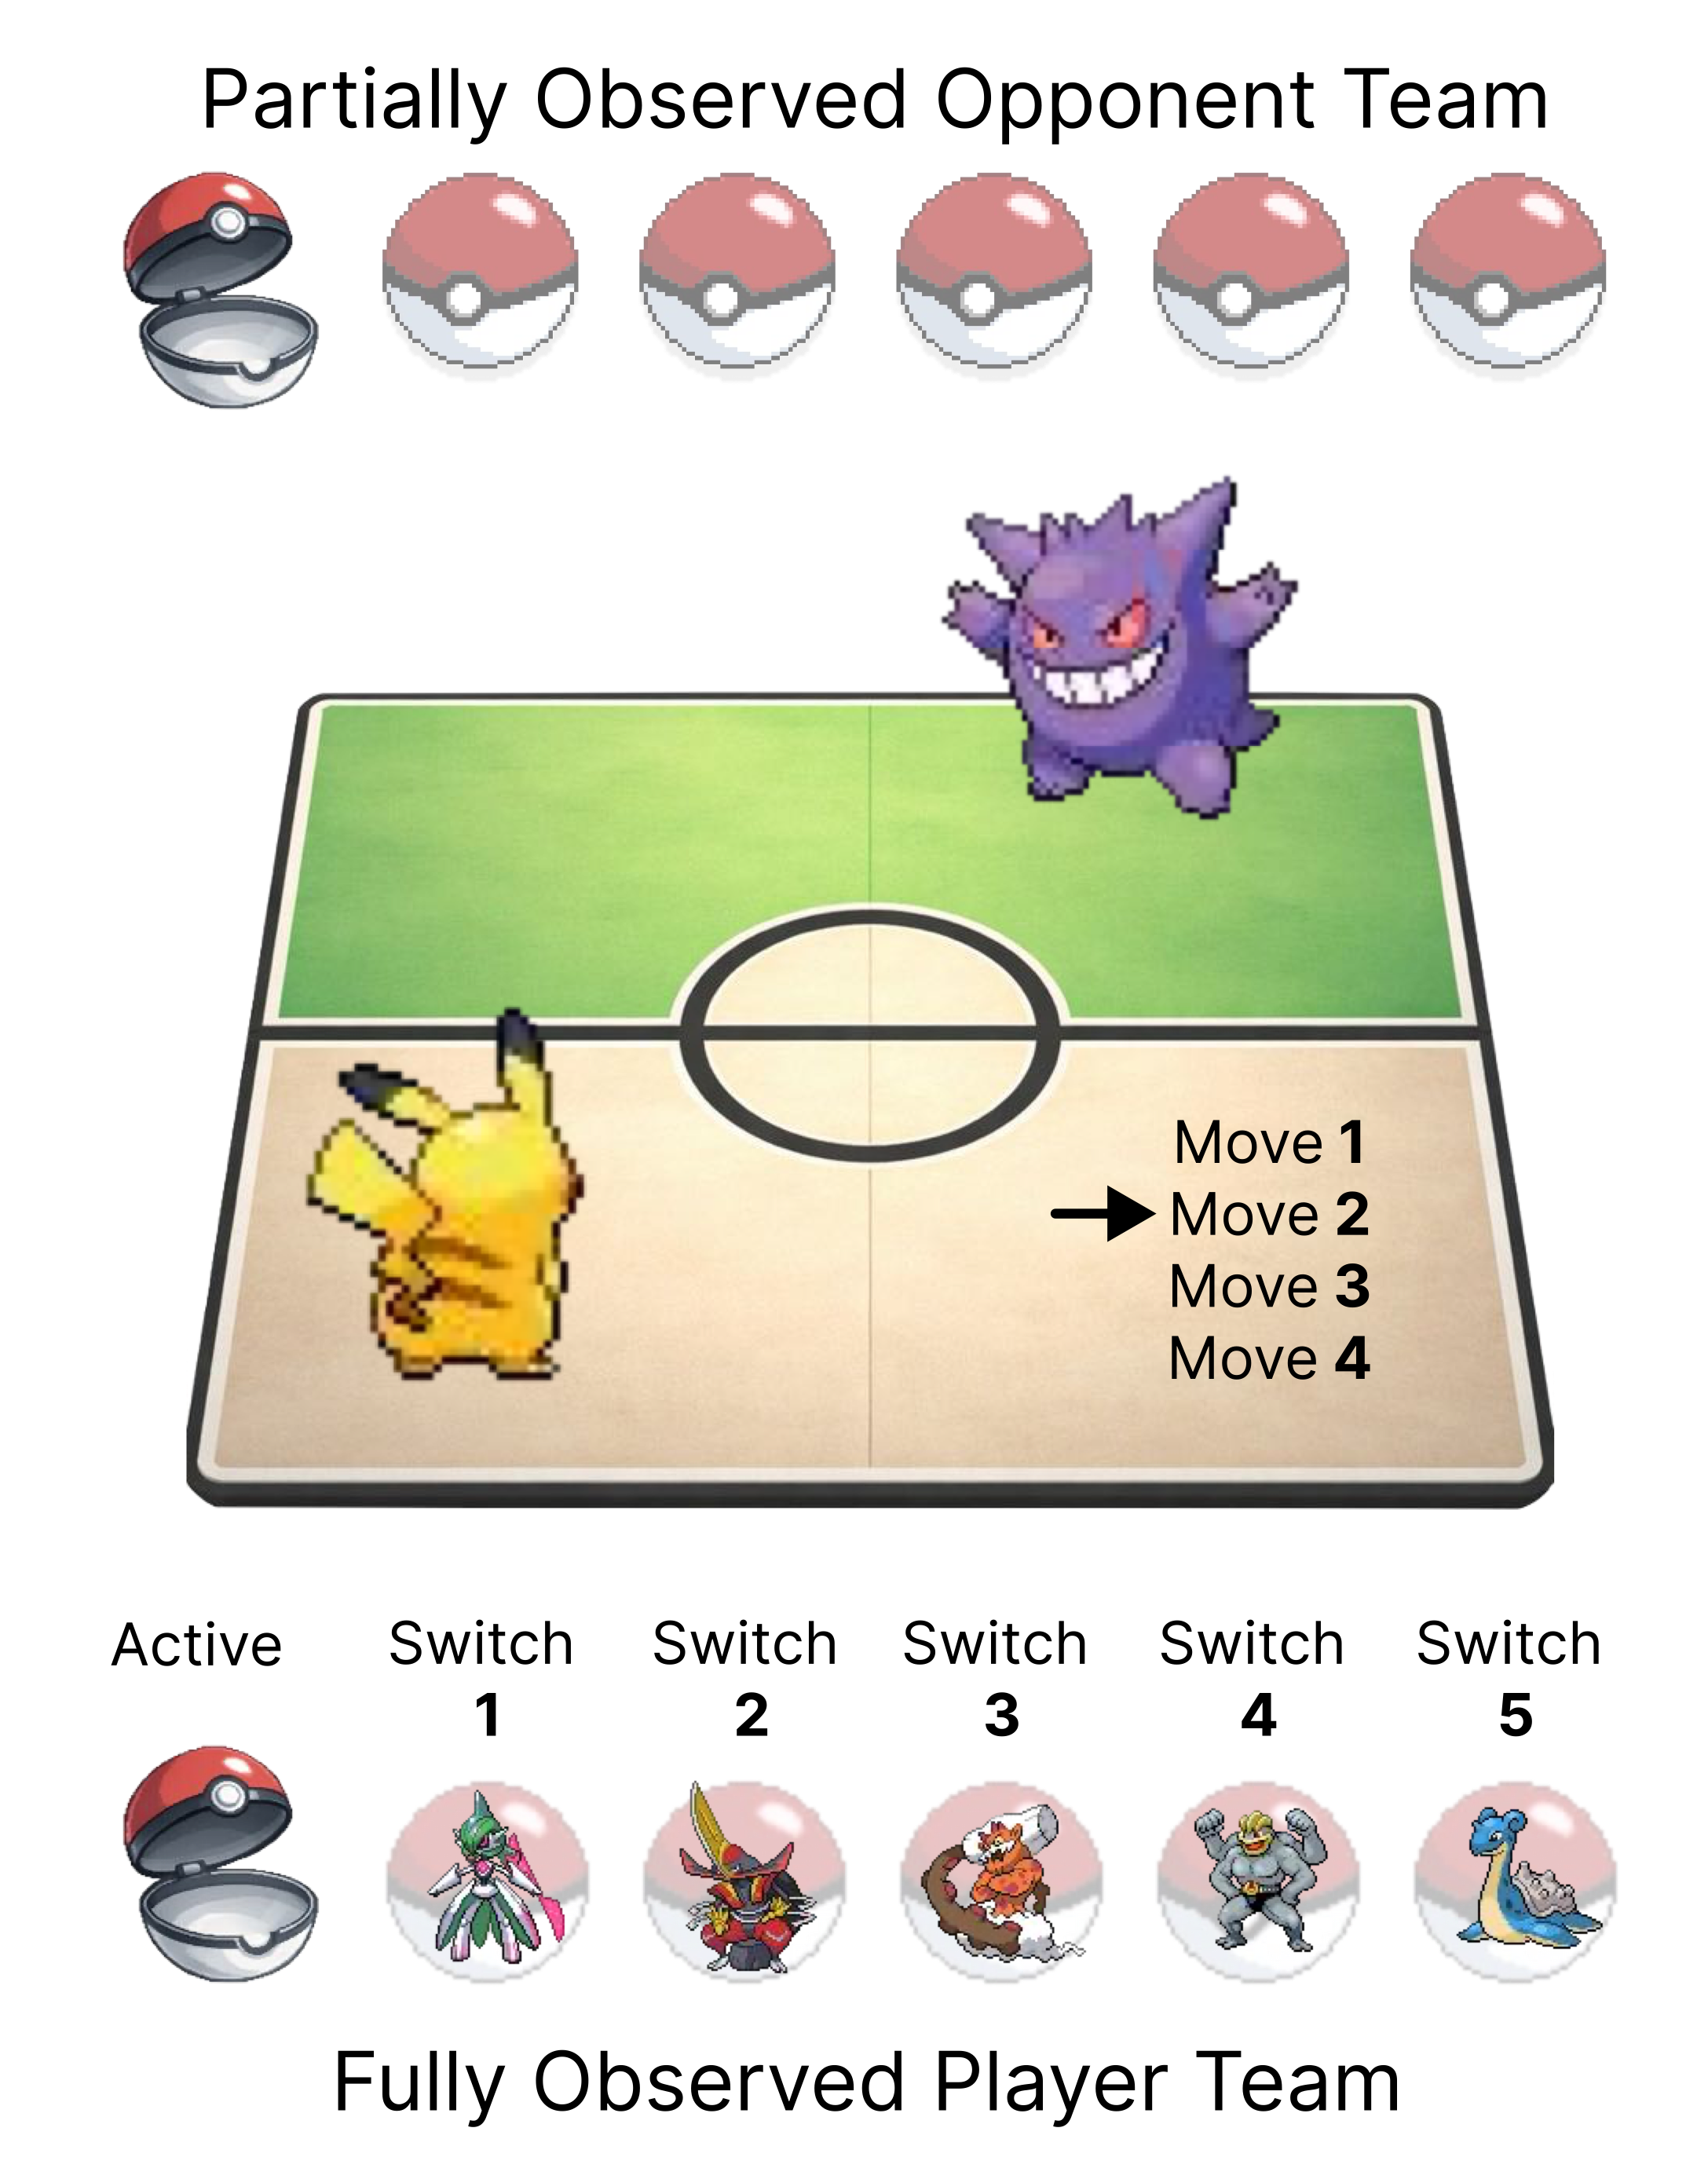
\includegraphics[width=.85\linewidth]{figures/battle_flattened_png.png}
    \vspace{-2mm}
    \caption{\textbf{Pokémon Battling.}}
    \vspace{-8mm}
    \label{fig:battle}
\end{wrapfigure}

\vspace{-2mm}

\paragraph{Rulesets.} Pokémon Showdown supports dozens of rulesets (``formats’’), but results here will focus on two that stress different AI capabilities: \textbf{Gen 1 OU} and \textbf{Gen 9 OU}. Gen 1 OU features greater effective hidden information and a more compact state space but yields smaller human demonstration datasets than Gen 9 OU. Our infrastructure currently supports three additional formats, with room to expand as performance saturates. Agents can play under two different time constraints: standard rules enforce faster-than-human play for efficient large-sample evaluation, while an ``Extended Timer'' variant provides nearly unlimited deliberation time for LLMs and test-time reasoning.

\subsection{Battling Baselines}

The PokéAgent Challenge is co-organized by the teams behind PokéChamp \cite{karten2025pok} and Metamon \cite{grigsby2025human}. While the Battling Track builds upon these leading LLM and RL approaches, the resources provided here have been heavily improved and standardized for this challenge. For clarity, we introduce these features as a unified framework, with novel improvements detailed in Appendix~\ref{sec:baseline-architectures}.


\paragraph{Demonstrations.} Showdown archives public battles spanning a decade of online play, and we organize an anonymized dataset of these files to protect player privacy. However, these ``replays'' are logged from a spectator’s perspective and do not reflect the private information available to each player at decision time. We release more than 4M RL trajectories generated by inferring private information and reconstructing the battle from each player’s perspective. The resulting dataset allows for flexible experimentation with alternative observation spaces, action spaces, and reward functions. While human demonstrations are invaluable for bootstrapping policies, competitive performance often requires the scale of self-play. We release all 18M trajectories used to train our strongest baselines and continue to expand this dataset with battles played on the PokéAgent Challenge server, including 100K community battles from our NeurIPS competition (Section~\ref{sec:neurips}).

\vspace{-2mm}


\paragraph{Sample Teams.} The combinatorial space of legal, competitively viable teams creates a substantial generalization challenge, as agents must perform across a vast range of initial conditions. Effective self-play training and evaluation demand diverse, realistic teams that mirror human trends. We release a dataset of 200K+ teams generated by inferring hidden information from human replays, alongside a curated collection of expert-validated teams sourced from community forums.

\begin{figure}[h!]
    \vspace{-2mm}
    \centering
    \makebox[\textwidth][c]{%
        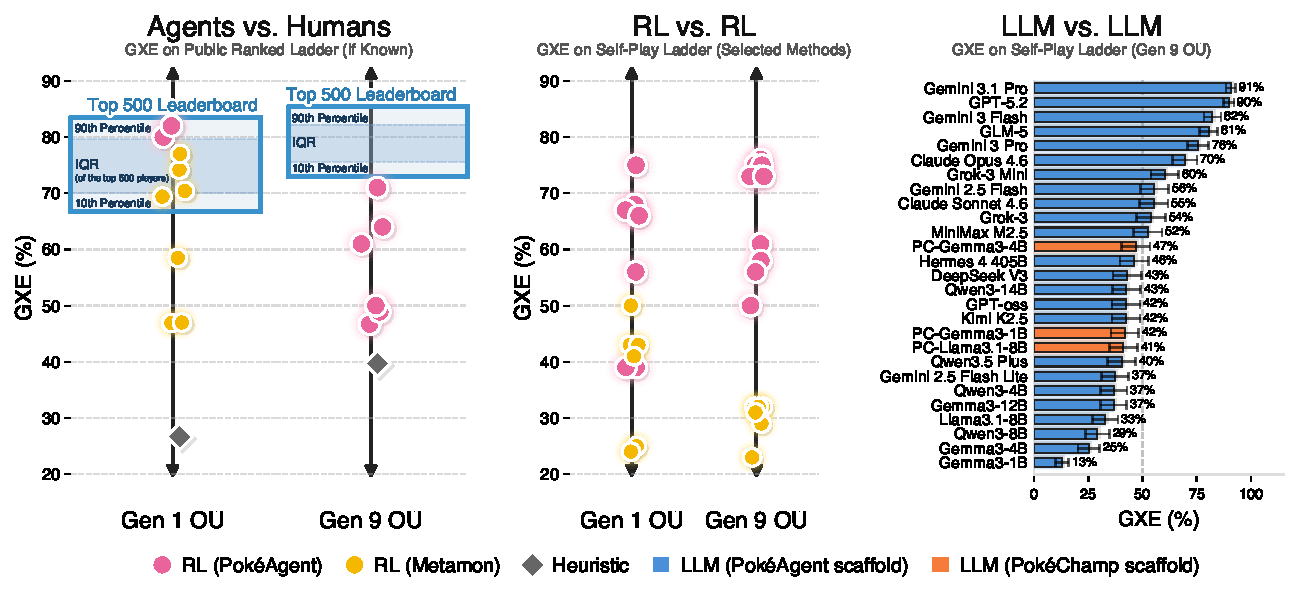
\includegraphics[width=1.02\textwidth]{figures/gxe_scatter.pdf}
    }
    \vspace{-7mm}
    \caption{\textbf{Baseline Performance.} \textbf{(Left) Agents vs. Humans}: Official ratings on the Showdown ladder. Statistics from the Top 500 leaderboard are provided as a frame of reference for experienced human players. \textbf{(Center/Right) RL vs. RL and LLM vs. LLM}: GXE is measured relative only to methods within each plot. We differentiate between prior Metamon RL policies \cite{grigsby2025human} and baselines newly developed for this work; \texttt{PC-Llama3.1-8B} represents the original PokéChamp agent \cite{karten2025pok}.}
    \label{fig:track1_baselines}
\end{figure}


\vspace{-2mm}

\paragraph{LLM Baselines.} Although Pokémon knowledge appears in pretraining corpora, competitive gameplay is not an explicit optimization target of LLM training, making the application of that knowledge in competitive battles a genuine out-of-distribution test that extends recent LLM evaluations in Chess and Poker~\cite{kaggle2025gamearena} to an even more complex domain. We extend PokéChamp~\cite{karten2025pok} into a generalized harness framework for reasoning models, supporting both frontier API models (GPT, Claude, Gemini) and open-source models (Llama, Gemma, Qwen). The framework converts game state to structured text and provides configurable harness including depth-limited minimax search with LLM-based position evaluation. All LLM baselines use a harness; even small open-source models achieve meaningful performance with this support (Figure~\ref{fig:track1_baselines}). Default turn timers (60--90s) proved insufficient for LLM inference; the Extended Timer setting provides nearly unlimited deliberation time for fair evaluation of these methods. See Appendix~\ref{sec:baseline-architectures} for architecture details.

\vspace{-2mm}

\paragraph{RL Baselines.} In competitive domains, specialized systems often set the performance ceiling before general-purpose approaches reach parity. Pokémon provides a venue to study this gap, and we include strong RL baselines trained on large datasets of human demonstrations and self-play battles. We extend Metamon \cite{grigsby2025human} and release checkpoints from 30 agents that span the competitive skill ladder, ranging from compact RNNs to 200M-parameter Transformers. Our RL baselines provide high-quality reference points across a range of human skill levels, allowing researchers to benchmark their progress and explore compute-efficiency tradeoffs on accessible hardware.



Figure \ref{fig:track1_baselines} visualizes the relative strength of select RL and LLM agents alongside their performance against human players on Pokémon Showdown. Our baselines represent a substantial improvement over prior work \cite{karten2025pok, grigsby2025human} and span a broad performance range in both categories, providing researchers with diverse reference points to track progress as they iterate on new techniques. The strongest baselines are competitive with top human players, confirming the benchmark captures the strategic depth of high-level play, though our current upper bound remains less than superhuman.